\section{Evaluation}
\label{sec:Evaluation}
In this section, we present the experimental settings and the evaluation results of the proposed \sys.

\subsection{Experimental Settings}
\subsubsection{Datasets}
We evaluate the proposed \sys on two public datasets CIC-IDS2017 dataset~\cite{sharafaldin2018toward} and ISCXVPN2016 traffic dataset~\cite{draper2016characterization}, respectively. 
The first dataset contains the hybrid of encrypted and unencrypted network traffic across five days, which can be divided into 8 classes, Benign, FTP Patator, SSH Patator, DoS, Web Brute Force, Botnet, Port Scan, and DDoS respectively.
The second dataset contains pure encrypted traffic, which is composed of 14 applications, \eg Facebook, Netflix, Skype, etc.
The applications are encrypted with various security protocols, including HTTPS, SSH, and proprietary protocols.
Both two datasets are imbalanced.
For example, in the CIC-IDS2017 dataset, Port Scan accounts for 35.07\%, while Botnet only accounts for 0.27\%.
In the ISCXVPN2016 traffic dataset, Email accounts for 16.89\%, while SFTP only accounts for 0.65\%. 

\subsubsection{Baselines}
We compare \sys against various baseline works for encrypted traffic classification, including KNN~\cite{mcgaughey2018systematic}, RF~\cite{zhai2018random}, MLP~\cite{aceto2018mobile}, LSTM~\cite{vu2018time}, and FS-Net~\cite{liu2019fs}. 

We compare our global feature ranking method against the mutual information feature ranking~\cite{kraskov2004estimating}, RFE feature ranking~\cite{guyon2002gene}, and random forest feature ranking~\cite{louppe2014understanding}.  
Since these methods cannot be performed on time-series features directly, we first reshape the time-series data into tabular data as mentioned in Section~\ref{sec:Sequence_Feature_Ranking}.
Then we calculate the feature importance on the reshaped data with these methods respectively.  
Finally, we \emph{restore} the results of feature importance to the corresponding time-series features to obtain the feature ranking of the original features.
The process \emph{restore} is to accumulate the feature importance of corresponding features on the reshaped data, for each feature of the original time-series data.

In terms of local interpretability, we compare the performance of our proposed method against well-known methods, including LIME~\cite{lime}, SHAP~\cite{shap}, and Feature Permutation~\cite{altmann2010permutation}.

\subsubsection{Implementation Details}
The time sequence length of each LSTM unit is set as 32.  
We set the dimension of the encoding layer as 8.
The dimension of hidden states of each fingerprint LSTM is set as 16.
The Adam optimizer~\cite{kingma2014adam} with a learning rate of 0.001 is used.  
Our proposed method \sys is implemented with \emph{PyTorch}. %~\cite{paszke2019pytorch}.
We use \emph{scikit-learn}~\cite{scikit-learn} to implement other compared methods.
The compared local interpretability methods are the implementation from \emph{Captum}~\cite{kokhlikyan2020captum}.
All experiments in this paper are conducted using a 12-core PC with an NVIDIA GeForce GTX 1070 GPU, 128GB of RAM, and Ubuntu 16.04 LTS.

\subsubsection{Evaluation Metrics}
We evaluate the classification performance of \sys with other baselines in terms of Accuracy (AC), Precision (PR), Recall (RC), and F1-Score (F1)~\cite{zheng2020learning}.
Macro Average~\cite{liu2017efficient} is used to avoid biased results due to imbalance between multiple categories of data by calculating the mean value of AC, PR, RC, and F1 of each category.

The performance of local interpretability will be evaluated in terms of stability, robustness, and effectiveness~\cite{fan2020can}.

\subsection{Evaluation of Classification}
In this section, we evaluate \sys and baseline classification methods with the 5-fold cross-validation.

\subsubsection{Effectiveness of the Fingerprint Learning}
\begin{figure*}[htbp]
	\centering
	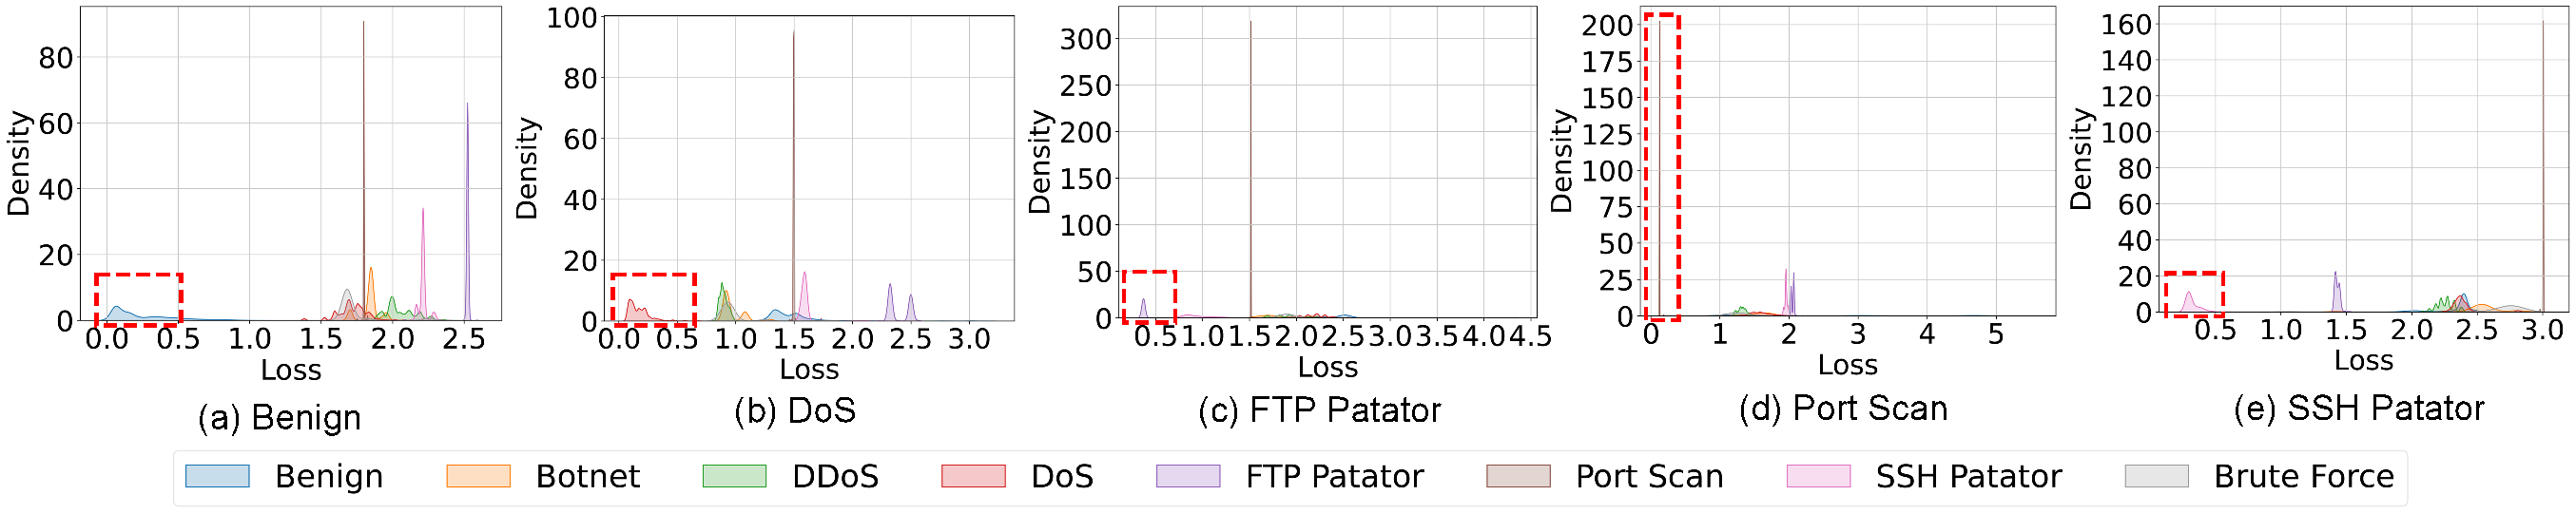
\includegraphics[scale=0.4]{figs/loss_kde.pdf}
	\caption{KDE of losses output by fingerprint modules when feeding different types of traffic data on CIC-IDS2017.}
	\label{fig:loss_kde}
\end{figure*}
In order to show the effectiveness of fingerprint learning, we plot the distribution of losses output by each fingerprint module when feeding traffic data of different types.
Each subfigure in Fig.~\ref{fig:loss_kde} shows the kernel density estimation (KDE)~\cite{silverman2018density} of the distribution of losses (due to page limitation we do not show all results).
The losses of samples whose types are exactly the corresponding type of the fingerprint module (red rectangle part) are significantly lower than that of other types (x-axis). 
It demonstrates that each fingerprint module in the fingerprint list of \sys can learn the \emph{fingerprint} of the corresponding traffic type well. 
In other words, the core idea of \sys described in Section~\ref{sec:Proposed_Traffic_Classification_Method} is effective. 

Table~\ref{tab:classification_ids} and Table~\ref{tab:classification_vpn} show the classification results. 
It is clear that \sys achieves significant classification performance and outperforms all other methods in both traffic datasets.
The KNN, RF, and MLP are designed to learn from the tabular data. 
They cannot model the context information in the sequence data and thus perform worse than \sys.
The \sys has a better classification performance than LSTM and FS-Net, especially in F1-Score.
It is mainly because both datasets are imbalanced.
The \sys leverages the advantage of fingerprint learning, \ie each fingerprint module is only responsible for identifying one traffic type. 
Thus it will not be confused by different traffic fingerprints and is suitable for imbalanced data. 

\begin{table}[htbp]
\centering
\caption{Comparison Results of Different Classification Methods on CIC-IDS2017 dataset}
\label{tab:classification_ids}
\begin{tabular}{|c|c|c|c|c|} 
\hline
Method       & AC     & PR     & RC     & F1     \\
\hline
\textbf{I2RNN}        & \textbf{0.9897} & \textbf{0.9864} & \textbf{0.9859} & \textbf{0.9861} \\
\textbf{I2RNN w/o EL} & 0.9769 & 0.9752 & 0.9729 & 0.9766 \\
\hline
KNN~\cite{mcgaughey2018systematic}          & 0.9579 & 0.8886 & 0.8891 & 0.8886 \\
RF~\cite{zhai2018random}           & 0.9698 & 0.9692 & 0.9621 & 0.9629 \\
MLP~\cite{aceto2018mobile}          & 0.9699 & 0.9699 & 0.9693 & 0.9630 \\
LSTM~\cite{vu2018time}         & 0.9649 & 0.7961 & 0.8560 & 0.8124 \\
FS-Net~\cite{liu2019fs}       & 0.9526 & 0.4721 & 0.4439 & 0.4218 \\
\hline
\end{tabular}
\end{table}

\begin{table}[htbp]
\centering
\caption{Comparison Results of Different Classification Methods on ISCXVPN2016 dataset}
\label{tab:classification_vpn}
\begin{tabular}{|c|c|c|c|c|}
\hline
Method       & AC     & PR     & RC     & F1     \\
\hline
\textbf{I2RNN}        & \textbf{0.9393} & \textbf{0.9068} & \textbf{0.9178} & \textbf{0.9013} \\
\textbf{I2RNN w/o EL} & 0.8922 & 0.8683 & 0.8693 & 0.8490 \\
\hline
KNN~\cite{mcgaughey2018systematic}          & 0.8799 & 0.7692 & 0.7094 & 0.6924 \\
RF~\cite{zhai2018random}           & 0.8712 & 0.8742 & 0.8647 & 0.8634 \\
MLP~\cite{aceto2018mobile}          & 0.8503 & 0.6992 & 0.6745 & 0.5540 \\
LSTM~\cite{vu2018time}         & 0.8813 & 0.5213 & 0.5132 & 0.5006 \\
FS-Net~\cite{liu2019fs}       & 0.5230 & 0.0924 & 0.1122 & 0.0859 \\
\hline
\end{tabular}
\end{table}

\subsubsection{Local Robustness of the Fingerprint Learning}
We compare the local robustness of the fingerprint learning of \sys and traditional classification with LSTM when having noise in packet sequence.
We add a Gaussian noise $\epsilon~N(0, 1)$ with different perturbation ratios $\beta \in [0, 1]$ to the last two packets in the packet sequence of a session.
The experiment results are shown in Fig.~\ref{fig:perturbation}.
When gradually increasing the perturbation ratio from 0.0 to 1.0, we find the accuracy and F1-Score of the fingerprint LSTM change slightly while the performance of the traditional LSTM drops sharply. 
This result indicates our fingerprint LSTM has local robustness and is more stable in face of noises in sessions.
\begin{figure}[htbp]
	\centering
	\subfloat{
		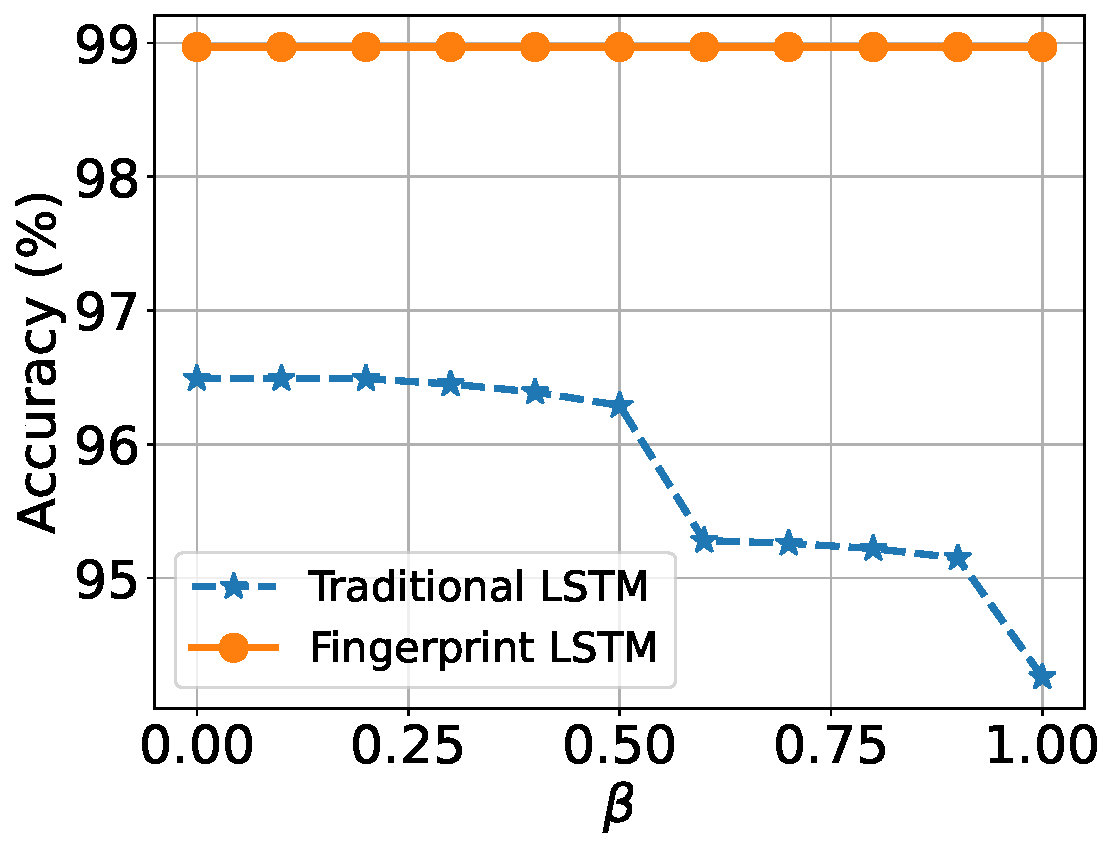
\includegraphics[width=0.47\linewidth]{figs/ids_perturbation_acc.pdf}
	}\hfill
	\subfloat{
		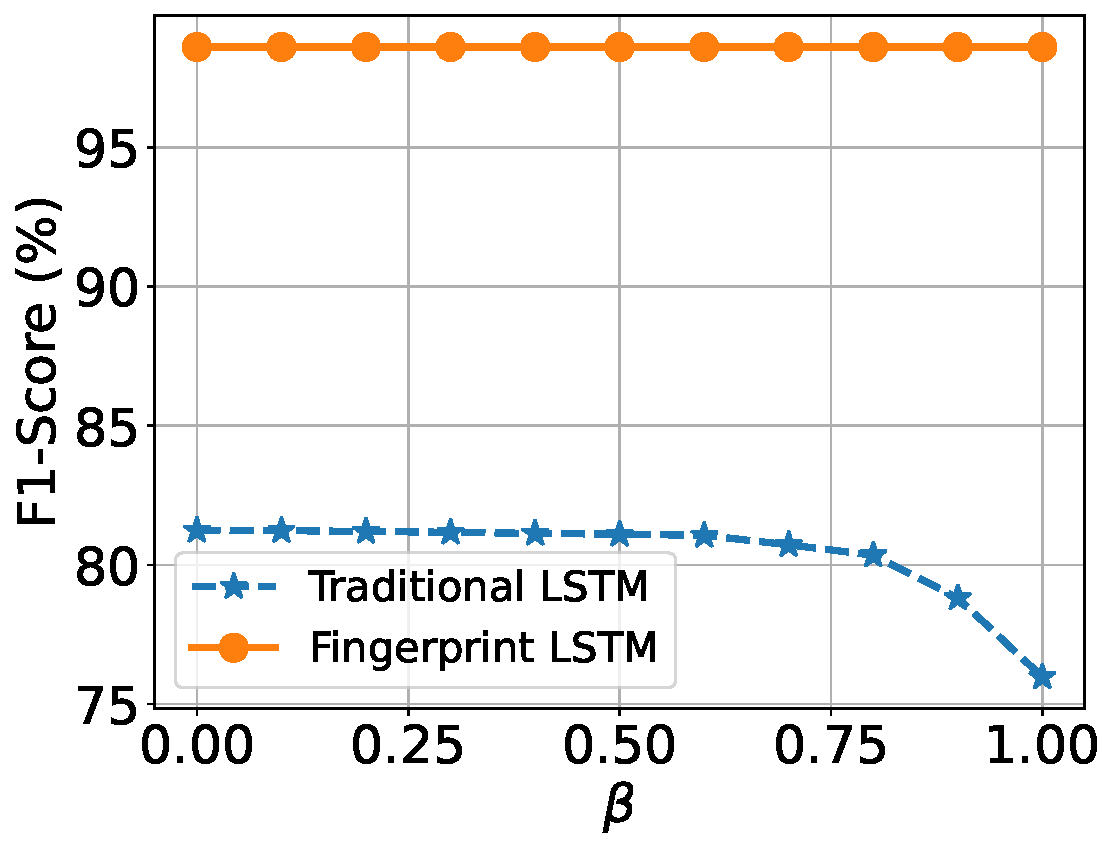
\includegraphics[width=0.47\linewidth]{figs/ids_perturbation_f1.pdf}
	}
	\caption{Comparison results of traditional LSTM and fingerprint LSTM on CIC-IDS2017 with different perturbation ratios $\beta$.}
	\label{fig:perturbation}
\end{figure}

\subsubsection{Ablation Study of the Encoding Layer}
To verify the effectiveness of the encoding layer, we train a variant version of \sys without the encoding layer (EL), which is termed as \sys w/o EL in Table~\ref{tab:classification_ids} and Table~\ref{tab:classification_vpn}.
We can see that the \sys with the encoding layer has a better performance than the variant version of \sys without the encoding layer. 
This result indicates that the encoding layer has effects on categorical feature transformation and redundant information reduction. 

\subsection{Evaluation of Incremental Learning}

\subsubsection{Comparison of Training Time and Preserved Data Size}
\label{sec:inc_time_size}
Fig.~\ref{fig:inc_time_size} presents the comparison of the training time and the size of data needed to be preserved when giving different numbers of incremental data.
Compared to the traditional LSTM, our proposed fingerprint LSTM is more efficient in training time and the size of data needed to be preserved under an incremental learning scenario. 

\begin{figure}[htbp]
	\centering
	\subfloat{
		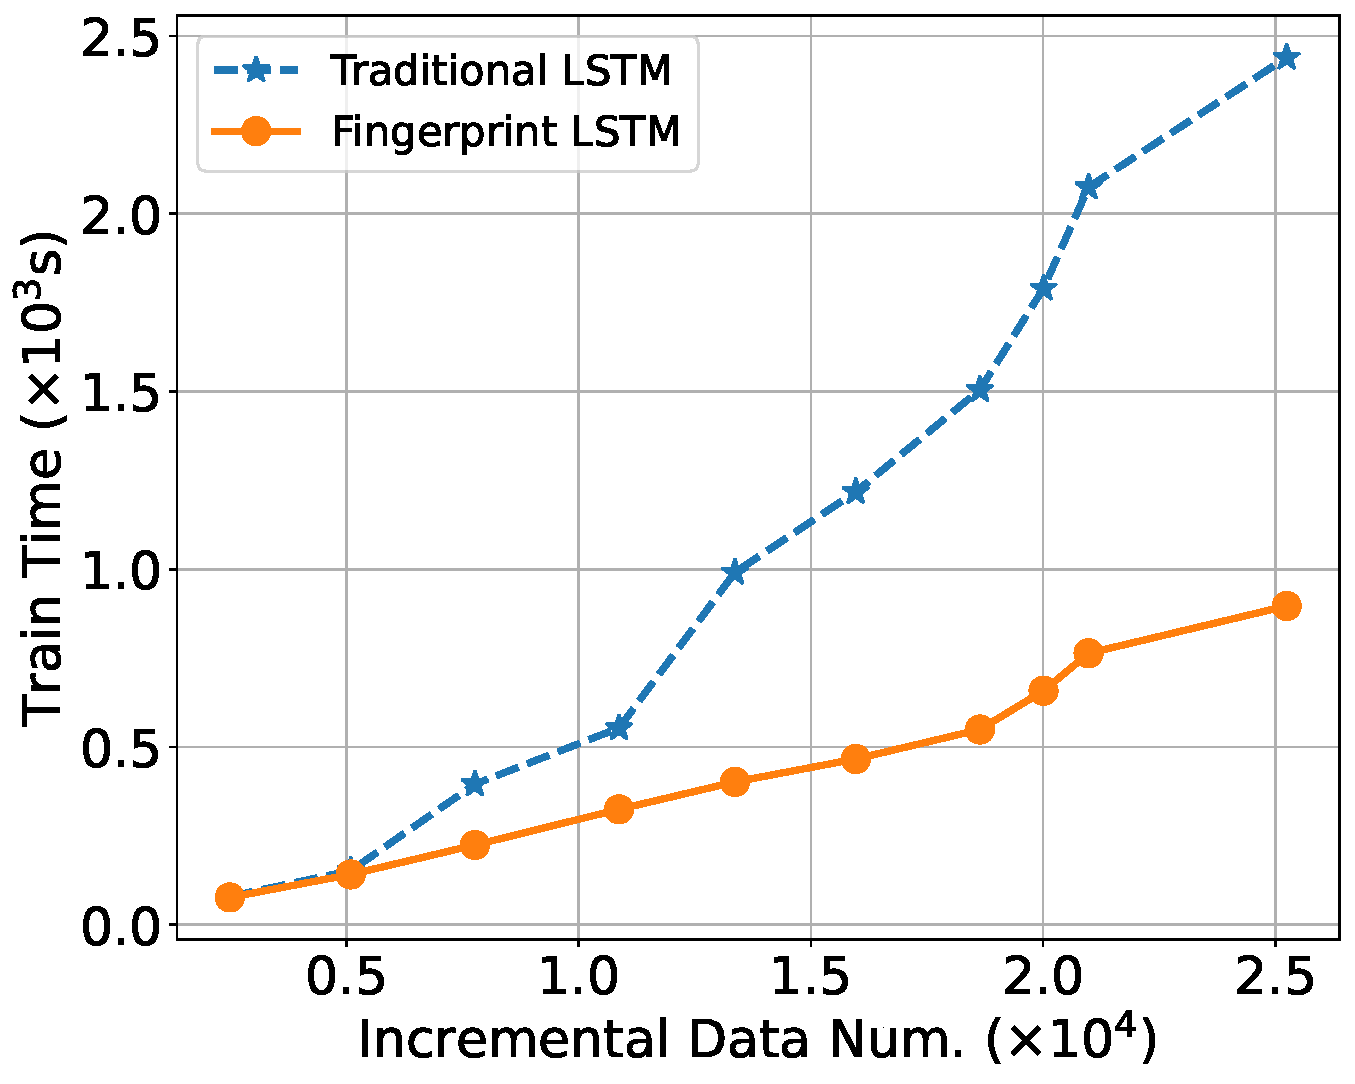
\includegraphics[width=0.47\linewidth]{figs/inc_time_size_cmp_time.pdf}
	}\hfill
	\subfloat{
		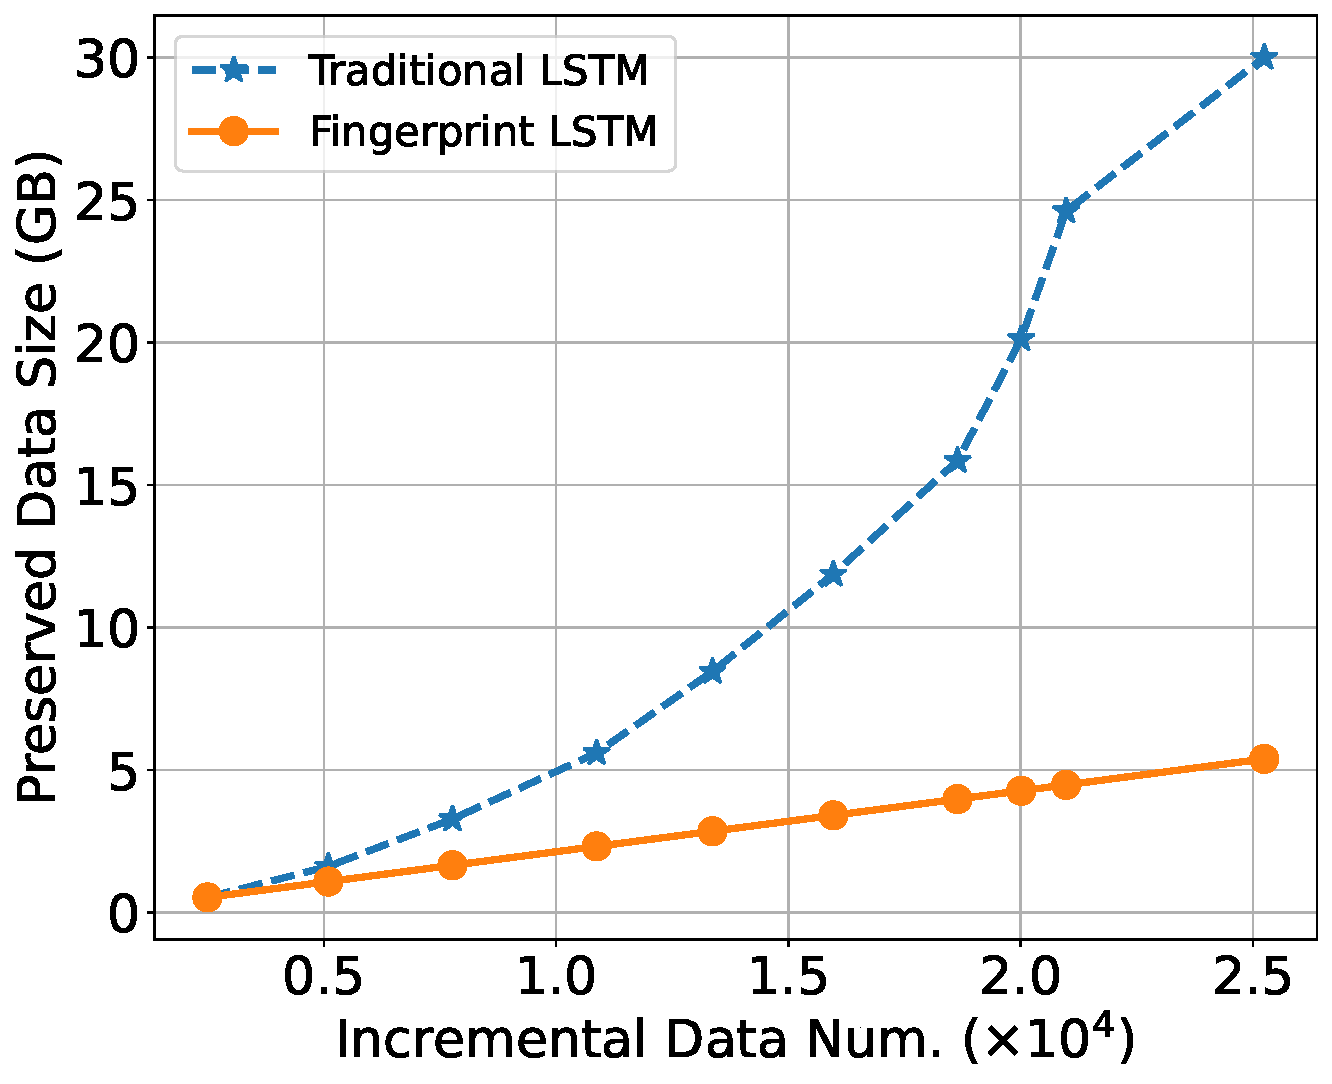
\includegraphics[width=0.47\linewidth]{figs/inc_time_size_cmp_size.pdf}
	}
	\caption{Comparison of training time and size of data needed to be preserved with different numbers of incremental data.}
	\label{fig:inc_time_size}
\end{figure}

\subsubsection{Classification Performance in Different Incremental Scenario}
We verify the classification performance of \sys under different incremental learning scenarios.
We consider three incremental scenarios including the addition of one traffic type, the addition of multiple traffic types at once, and the sequential addition of multiple traffic types.
We first sort the names of traffic types in alphabetical order.
In each incremental scenario, we select the first few traffic types as the incremental traffic types and the remaining traffic types as the initial types. 
Then we train the model to learn new traffic types according to the incremental scenarios. 
Table~\ref{tab:increment_experiment} shows the experiment results. 
In Table~\ref{tab:increment_experiment}, the symbol plus ($+$) means that the corresponding type is added for incremental learning.
The \emph{new} means traffic types newly added during incremental learning and the \emph{old} means traffic types before incremental learning. 
We observe that as long as the trained traffic types are the same (including those gradually added for incremental learning),  the performance of the \sys will be the same. 
This indicates that incremental learning of \sys has the same effect as the training model with full data at once.
In other words, our incremental learning algorithm of \sys does not cause a degradation in classification performance.  

\begin{table}[htbp]
	\centering
	\caption{Classification Performance (F1-Score) Under Different Incremental Learning Scenarios}		
	\label{tab:increment_experiment}
	\begin{tabular}{|c|c|c|c|}
	\hline
	Scenario                                                                                  & Total                   & New                     & Old                     \\ \hline
	+Benign                                                                                   & \textbf{0.9861}                  & 0.9899                  & 0.9855                  \\ 
	+Benign \& Botnet                                                                         & \textbf{0.9861}                  & 0.9886                  & 0.9852                  \\ 
	\multirow{2}{*}{\begin{tabular}[c]{@{}c@{}}+Benign \& Botnet\\ $\rightarrow$+DDoS \& DoS\end{tabular}} & \multirow{2}{*}{\textbf{0.9861}} & \multirow{2}{*}{0.9891} & \multirow{2}{*}{0.9829} \\
	                                                                                          &                         &                         &                         \\ \hline
	\end{tabular}
\end{table}

\subsection{Evaluation of Interpretability}
For the model interpretability of \sys, we first evaluate the global and local interpretability respectively, and then the effectiveness of inter-class distance.
\subsubsection{Effectiveness of Global Feature Ranking}
To examine the effectiveness of features ranked by different methods, we first partition the ranked features into two equal groups, that is, each group has 8 features. 
Then we use features in each group to classify the traffic.
The results are shown in Fig.~\ref{fig:feature_rank_cmp_group}.
We can observe that the first group of \sys has a better F1-Score than the second group.
This indicates that the feature ranking of \sys is effective.
Moreover, we validate the effectiveness of feature ranking by selecting a different number of features according to feature ranking results to perform classification tasks. 
Fig.~\ref{fig:feature_rank_cmp_num_acc}~and~\ref{fig:feature_rank_cmp_num_f1} show the experiment results. 
Compared with other feature ranking methods, our method can achieve higher classification performance with the same number of features. 
This suggests that our feature ranking method can choose the important features of time-series data and is more effective than other feature ranking methods. 
Particularly, using our feature ranking method can achieve classification performance similar to using all features with only half the number of original features. 
Finally, we also compare the time cost of different feature ranking methods and the results are shown in Fig.~\ref{fig:feature_rank_cmp_time}.
We can see that \sys uses the shortest time to rank features while other methods need a longer time to handle or are even impossible to get results in a tolerable time (see a red cross in RFE).
We argue that the efficiency of the feature ranking method is also a part of the interpretable evaluation, which allows users to have quick feedback and a good user experience. 

\begin{figure}[htbp]
	\centering
	\subfloat[]{
		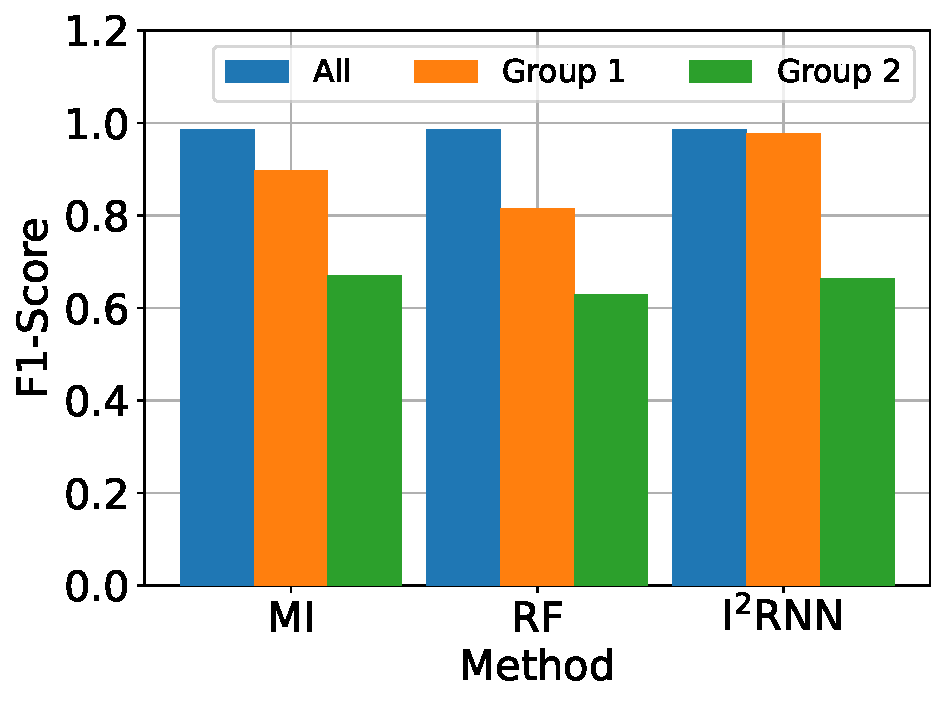
\includegraphics[width=0.47\linewidth]{figs/fea_rank_cmp_group.pdf}
		\label{fig:feature_rank_cmp_group}
	}\hfill
	\subfloat[]{
		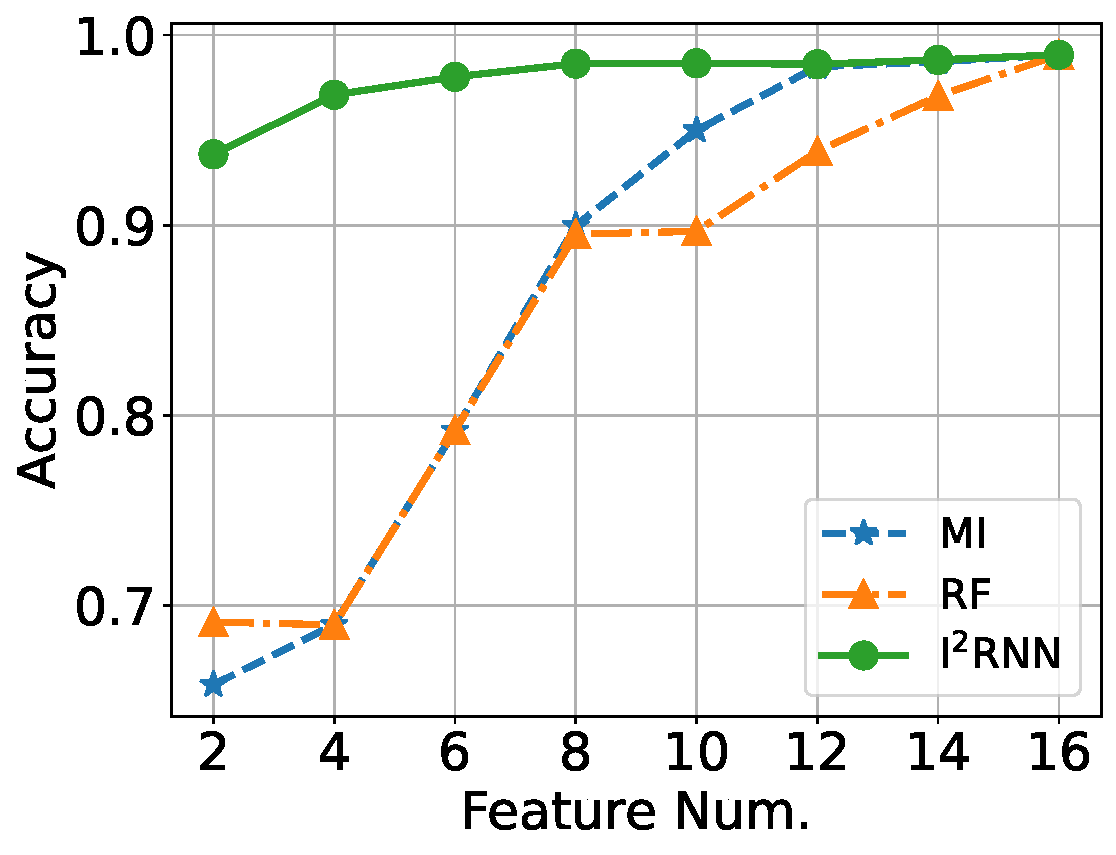
\includegraphics[width=0.47\linewidth]{figs/fea_rank_cmp_num_acc.pdf}
		\label{fig:feature_rank_cmp_num_acc}
	}\\
	\subfloat[]{
		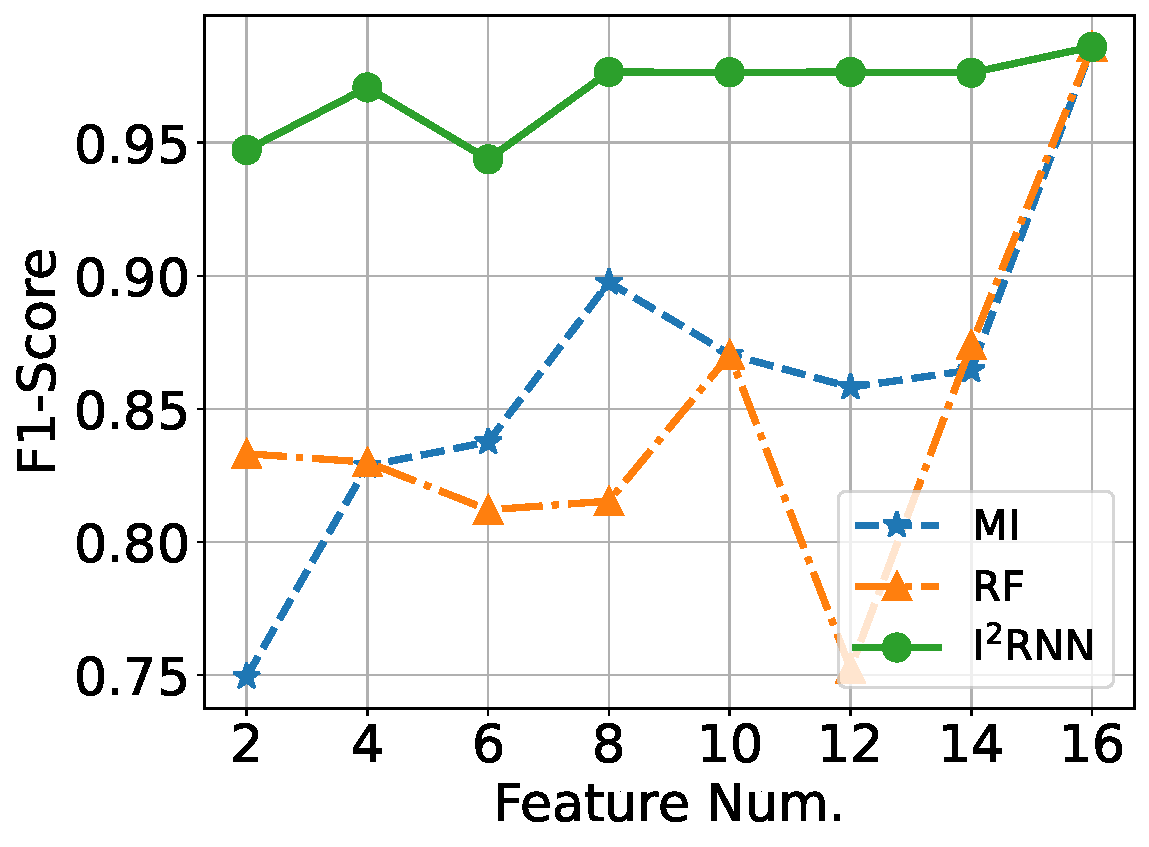
\includegraphics[width=0.47\linewidth]{figs/fea_rank_cmp_num_f1.pdf}
		\label{fig:feature_rank_cmp_num_f1}
	}\hfill
	\subfloat[]{
		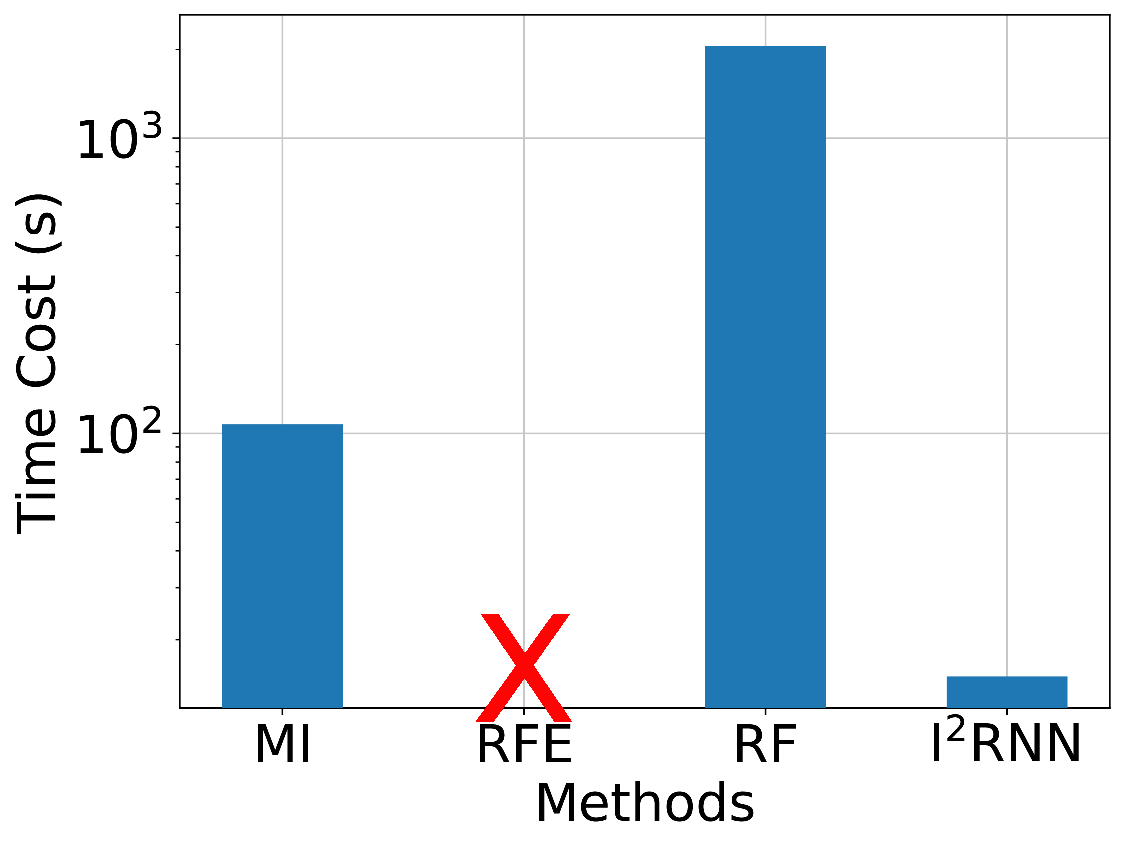
\includegraphics[width=0.47\linewidth]{figs/fea_rank_cmp_time.pdf}
		\label{fig:feature_rank_cmp_time}
	}
	\caption{Experiment results of global model interpretability.}
	\label{fig:experiment_results_interpretability}
\end{figure}

\subsubsection{Performance Comparison of Local Interpretability}
We compare the performance of the local interpretability of \sys with LIME~\cite{lime}, SHAP~\cite{shap}, and feature permutation (PERM)~\cite{altmann2010permutation} in terms of stability, robustness, and effectiveness~\cite{fan2020can}. 
Stability is the fundamental metric of local interpretability. 
The explanation results generated in a critical security system should be stable. 
That is, the feature importance must not be seriously influenced by the slight fluctuation of the model (\eg n\_epochs = 95, n\_epochs = 100, and n\_epochs = 105). 
Robustness is used to measure how similar the explanation results are for similar instances, \ie the feature importance of samples of the same class should be similar, while the feature importance of samples of different classes should be as distinct as possible. 
Effectiveness is the measure of whether the explanation results are important to the decision-making. 
In other words, if the explanation results are really the decision basis for an individual prediction, then after the elimination of such features, the classification result would be changed. 

\begin{figure}[htbp]
	\centering
	\subfloat[Stability]{
		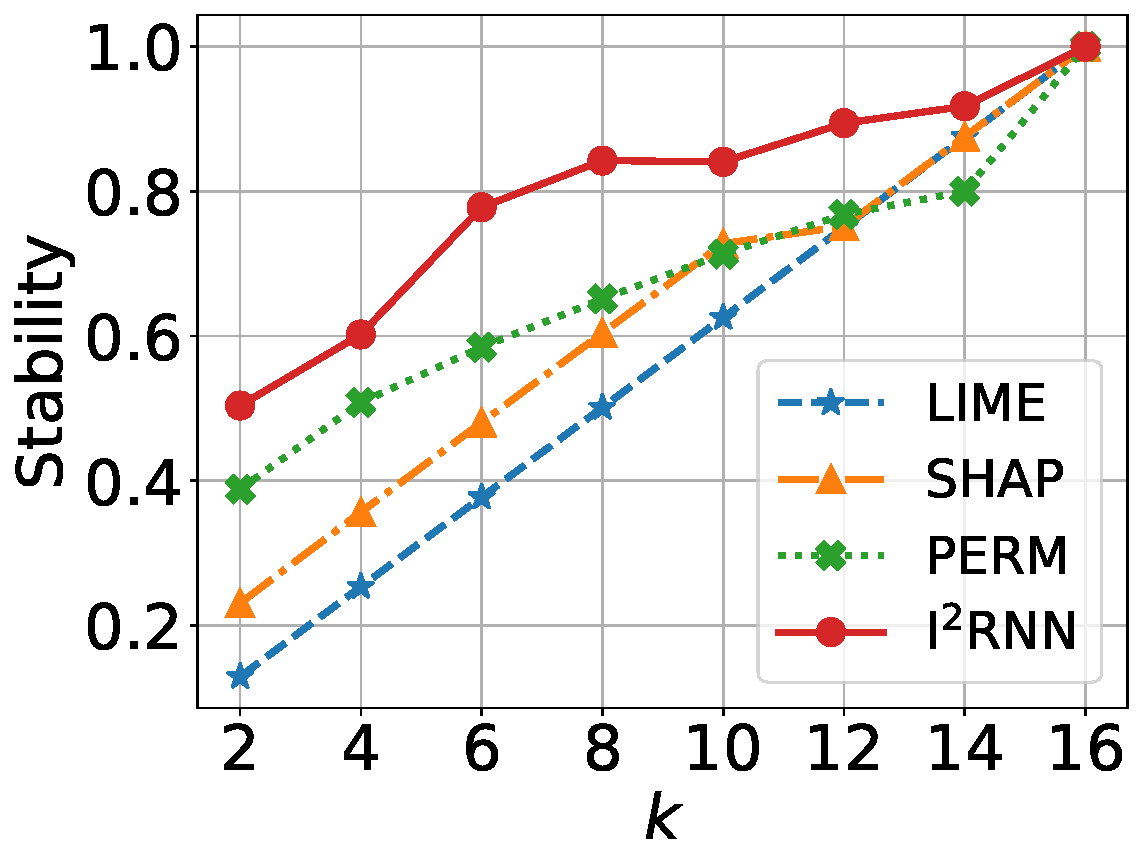
\includegraphics[width=0.47\linewidth]{figs/fea_local_cmp_stability.pdf}
		\label{fig:interpret_stability}
	}\hfill
	\subfloat[Robustness]{
		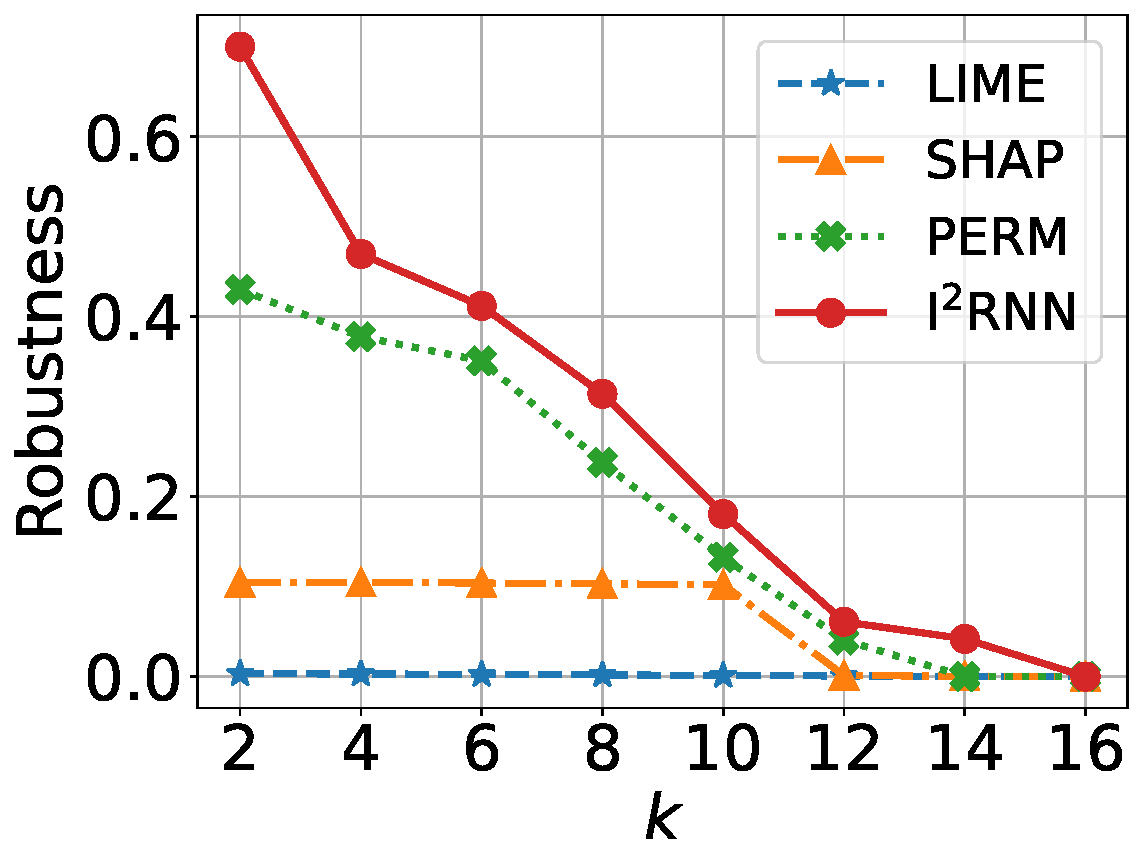
\includegraphics[width=0.47\linewidth]{figs/fea_local_cmp_robustness.pdf}
		\label{fig:interpret_robustness}
	}\hfill
	\subfloat[Effectiveness]{
		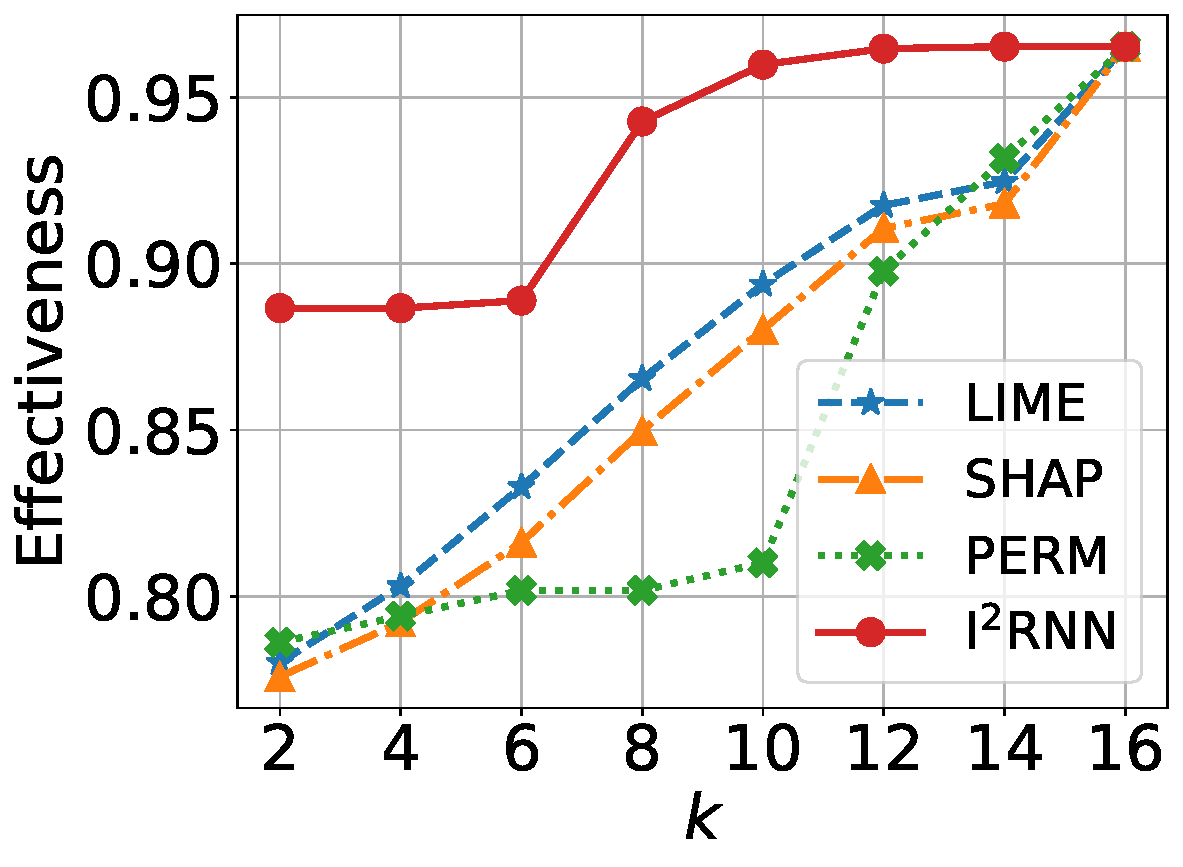
\includegraphics[width=0.47\linewidth]{figs/fea_local_cmp_effectiveness.pdf}
		\label{fig:interpret_effectiveness}
	}\hfill
	\caption{Performance comparison of local interpretability.}
	\label{fig:experiment_results_local_interpretability}
\end{figure}

Fig.~\ref{fig:experiment_results_local_interpretability} illustrates the performance comparison of local interpretability in terms of stability, robustness, and effectiveness under different top-$k$ features. 
From the figure, we can observe that:
\begin{itemize}
\item The \sys shows the best stability, robustness, and effectiveness compared to other methods under different top-$k$ features. 
\item The ranking of the four local interpretability approaches in term of the stability metric is \sys $>$ PERM $>$ SHAP $>$ LIME. The stability of \sys is above 0.8 when $k \ge 6$, indicating that explanation features hardly change when slightly modifying the model. 
\item The ranking of the four local interpretability approaches in term of the robustness metric is \sys $>$ PERM $>$ SHAP $>$ LIME. With the increase of $k$, the robustness of the four methods decreases. For SHAP and LIME, their robustness scores are lower than 0.2, and they hardly change under various $k$ values. The robustness of PERM is less than 0.5. These indicate that PERM, SHAP, and LIME cannot capture the core differences between traffic types especially when $k$ is small.
\item The ranking of the four local interpretability approaches in term of the effectiveness metric is \sys $>$ LIME $\ge$ SHAP $>$ PERM. The effectiveness of LIME and SHAP is very similar. For \sys, the effectiveness starts to be stable when $k > 8$. This indicates important features of \sys are in the top half of the ranked features, which results in little change of predicted label with higher $k$ values.
\end{itemize}

\subsubsection{Effectiveness of Inter-Class Distance}\label{sec:group}
To validate whether inter-class distance effectively characterizes the similarity between traffic types, we group traffic types with close distance as an individual traffic type. 
As depicted in Fig.~\ref{fig:traffic_distance}, Botnet and Brute Force are the closest in all features and thus we group them into an individual type. 
We also group DDoS and DoS which are close in all features. 
For a fair comparison (i.e., taking out the factor of category reduction), we also group traffic types with large distances. 
We group Port Scan and SSH Patator which are the farthest types in all features. 
Benign and DDoS are also grouped as an experiment for large distances. 
The results are shown in Table~\ref{tab:group_experiment}. 
We can observe that the performance is improved if we group traffic types that have small inter-class distances (i.e., they are close in some dimensions or in all features), while the performance significantly decreases if we group traffic types with large distances. 
These results indicate that our inter-class distance is rational, which captures the relationships between traffic types. 

\begin{table}[htbp]
	\centering
	\caption{Experiment Results of Different Grouping Strategies}		
	\label{tab:group_experiment}
	    \begin{tabular}{|c|c|c|c|}
	    \hline
	    Grouping Strategy & Distance & AC (\%) & F1 (\%) \\
	    \hline
	    \textbf{Botnet} \& \textbf{Brute Force} & \textbf{0.65} & \textbf{99.95} & \textbf{98.90} \\
	    \textbf{DDoS} \& \textbf{DoS} & \textbf{1.28} & \textbf{99.64} & \textbf{98.81} \\
	    \hline
	    Benign \& DDoS & 2.67 & 91.24 & 85.31 \\
           Port Scan \& SSH Patator & 7.49 & 79.71 & 80.84 \\
	    \hline
	    \end{tabular}
\end{table}